\documentclass[11pt]{article}

\usepackage{graphicx}

% Use wide margins, but not quite so wide as fullpage.sty
\marginparwidth 0.5in 
\oddsidemargin 0.25in 
\evensidemargin 0.25in 
\marginparsep 0.25in
\topmargin 0.25in 
\textwidth 6in \textheight 8 in
% That's about enough definitions


\begin{document}
\hfill\vbox{\hbox{Jude Shin, Torrey Zachs}
		\hbox{CSC 321, Section 07}	
		\hbox{Module 2: Block Ciphers}	
		\hbox{\today}}\par

\bigskip
\centerline{\Large\bf Lab 02: Symmetric Key Cryptography Exploration}\par
\bigskip

This lab explores symmetric key cryptography security with both Electronic Codebook (ECB) and Cipher Block Chaining (CBC) modes. This lab also demonstrates the limits and exploitations of each, as well as a performance study of public versus symmetric key algorithms. This lab was completed using {\tt Python} and {\tt PyCryptodome}.

\section*{Task 1: Modes of Operation}
\subsection*{Approach}
\subsection*{Problems Encountered}
\subsection*{Solutions}

\section*{Task 2: Limits of Confidentiality}
\subsection*{Approach}
\subsection*{Problems Encountered}
\subsection*{Solutions}

\section*{Task 3: Performance Comparison}
\begin{figure}
	\centering
	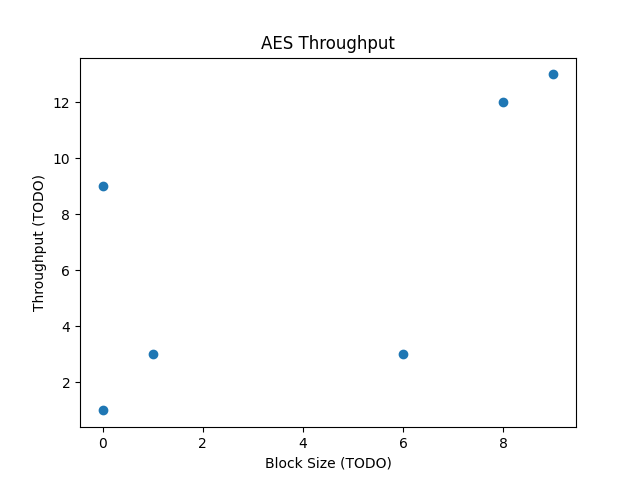
\includegraphics[width=0.8\textwidth]{./plts/aes.png}
	%\caption{}
	\label{fig.1: Performance of AES}
\end{figure}

\begin{figure}
	\centering
	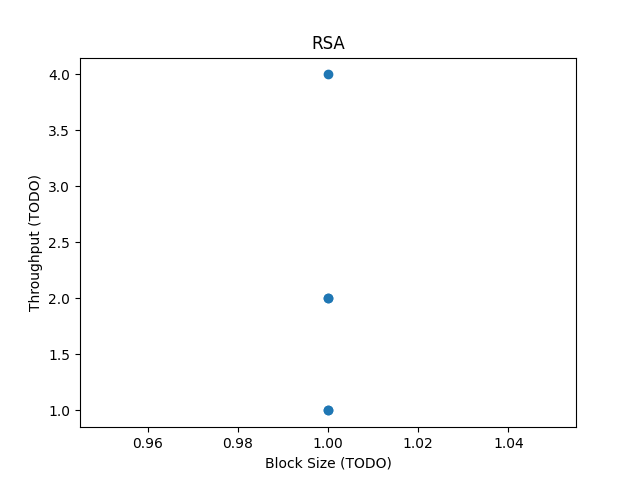
\includegraphics[width=0.8\textwidth]{./plts/rsa.png}
	%\caption{}
	\label{fig.2: Performance of RSA}
\end{figure}

\section*{Questions}
\subsection*{question 1}
\subsection*{question 2}
\subsection*{question 3}

\end{document}
